\documentclass[11pt,letter]{article}
\usepackage[utf8]{inputenc}
\usepackage{amsmath,amssymb,booktabs}
\usepackage[margin=2.3cm]{geometry}
\usepackage{xcolor,tcolorbox}
\usepackage{tikz,pgfplots}
\usepackage{listings}
\usepackage{hyperref}
\pgfplotsset{compat=1.18}
\hypersetup{hidelinks}
\definecolor{aggiemaroon}{RGB}{80,0,0}
\definecolor{teal}{RGB}{22,124,128}
\definecolor{gold}{RGB}{200,155,60}
\definecolor{lightteal}{RGB}{231,242,241}
\definecolor{lightgold}{RGB}{248,240,220}
\newcommand{\CFP}{C_{\mathrm{FP}}}
\newcommand{\CFN}{C_{\mathrm{FN}}}
\newtcolorbox{ideia}{colback=lightteal,colframe=teal,boxrule=0.7pt}
\newtcolorbox{atencao}{colback=lightgold,colframe=gold,boxrule=0.7pt}
\lstset{basicstyle=\ttfamily\small,frame=single,breaklines=true,showstringspaces=false}
\title{\textcolor{aggiemaroon}{Limiar de $\theta$ e Probabilidade Bayesiana}}
\author{DAEN 427 / ISEN 427 / ISEN 627\\
        Alexander Abuabara}
\date{\color{aggiemaroon}{Fall 2026}}

\begin{document}
\maketitle

\begin{ideia}
\textbf{Ideia principal:} primeiro definimos o que seria um processo
problemático. Depois usamos dados para calcular quão provável é que esse
problema exista. Finalmente, consideramos os custos dos possíveis erros para
decidir se devemos agir.
\end{ideia}

O objetivo é distinguir três quantidades:
\[
\boxed{\theta_0\qquad q=P(\theta>\theta_0\mid D)\qquad \tau}
\]

\section{A taxa verdadeira e seu limite}

Imagine uma fábrica de alimentos. Chamaremos de $\theta$ a verdadeira
proporção de itens contaminados:
\[
\theta=\text{verdadeira taxa de contaminação}.
\]
Se $\theta=0{,}10$, aproximadamente 10\% dos itens seriam contaminados em longo
prazo. O valor de $\theta$ é desconhecido porque não podemos testar todos os
itens produzidos no passado e no futuro.

A administração considera inaceitável uma taxa superior a 25\%. Esse limite é
\[
\theta_0=0{,}25.
\]
O estado adverso é
\[
\theta>\theta_0,
\]
ou, neste exemplo,
\[
\theta>0{,}25.
\]

\begin{ideia}
O número $0{,}25$ define quando a taxa verdadeira é considerada alta demais.
Ele ainda não informa a probabilidade de o problema existir.
\end{ideia}

\subsection{Analogia}

Um limite de velocidade de 80 km/h define o que conta como excesso de
velocidade, mas não informa a probabilidade de um carro estar acima do limite.
Da mesma forma, $\theta_0=0{,}25$ define o que conta como contaminação
excessiva, mas não informa a probabilidade de $\theta$ estar acima desse valor.

\section{A priori, os dados e a posterior}

Antes dos testes,
\[
\theta\sim\operatorname{Beta}(2,8).
\]
A fábrica testa 20 itens e encontra 8 contaminados. Existem 8 resultados
positivos e 12 negativos. Pela atualização Beta--Binomial,
\[
\theta\mid D
\sim\operatorname{Beta}(2+8,8+12)
=\operatorname{Beta}(10,20).
\]
O símbolo $D$ representa os dados observados. A expressão $\theta\mid D$
significa a distribuição de $\theta$ depois de considerarmos os dados.

A proporção observada é
\[
\frac{8}{20}=0{,}40,
\]
enquanto a média posterior é
\[
E(\theta\mid D)=\frac{10}{10+20}=0{,}3333.
\]

\begin{atencao}
A média posterior não responde diretamente à pergunta sobre a probabilidade de
$\theta$ ser maior que $0{,}25$. Precisamos considerar toda a distribuição.
\end{atencao}

\section{A probabilidade bayesiana $q$}

Como $\theta$ é desconhecido, calculamos
\[
q=P(\theta>0{,}25\mid D).
\]
Essa é a probabilidade de a verdadeira taxa de contaminação ser superior a
25\%, considerando os dados observados.
\subsection{Gráfico da distribuição posterior}

\begin{figure}[ht]
\centering
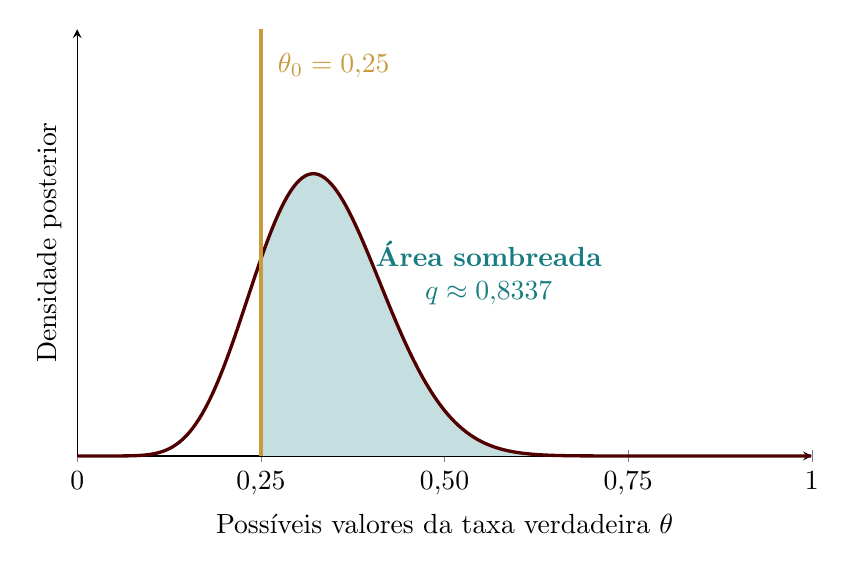
\begin{tikzpicture}
\begin{axis}[
  width=0.90\textwidth,
  height=7cm,
  xmin=0, xmax=1, ymin=0,
  axis lines=left,
  xlabel={Possíveis valores da taxa verdadeira $\theta$},
  ylabel={Densidade posterior},
  xtick={0,0.25,0.5,0.75,1},
  xticklabels={$0$,$0{,}25$,$0{,}50$,$0{,}75$,$1$},
  ytick=\empty,
  samples=250,
  domain=0.001:0.999,
  clip=false
]
\addplot[draw=none,fill=teal!25,domain=0.25:0.999]
  {200300100*x^9*(1-x)^19} \closedcycle;
\addplot[very thick,aggiemaroon,domain=0.001:0.999]
  {200300100*x^9*(1-x)^19};
\addplot[very thick,gold] coordinates {(0.25,0) (0.25,7)};
\node[anchor=west,text=gold,font=\bfseries]
  at (axis cs:0.26,6.4) {$\theta_0=0{,}25$};
\node[align=center,text=teal,font=\bfseries]
  at (axis cs:0.56,3.0) {Área sombreada\\$q\approx0{,}8337$};
\end{axis}
\end{tikzpicture}
\caption{Distribuição posterior $\operatorname{Beta}(10,20)$. A região
sombreada representa $P(\theta>0{,}25\mid D)$.}
\end{figure}

A área sombreada é
\[
q=P(\theta>0{,}25\mid D)\approx0{,}8337.
\]

\begin{ideia}
Dados o modelo, a priori e os testes, atribuímos probabilidade posterior de
83,37\% à afirmação de que a verdadeira taxa excede 25\%.
\end{ideia}

\section{Como calcular $q$}

A função acumulada informa a probabilidade de $\theta$ estar à esquerda:
\[
F_{\operatorname{Beta}(10,20)}(0{,}25)
=P(\theta\leq0{,}25\mid D)
\approx0{,}166305.
\]
Como queremos a área à direita,
\[
P(\theta>0{,}25\mid D)=1-P(\theta\leq0{,}25\mid D).
\]
Portanto,
\[
q=1-0{,}166305=0{,}833695\approx0{,}8337.
\]

\subsection{Cálculo em R}

\begin{lstlisting}[language=R]
pbeta(
  0.25,
  shape1 = 10,
  shape2 = 20,
  lower.tail = FALSE
)
\end{lstlisting}

\subsection{Cálculo em Python}

\begin{lstlisting}[language=Python]
from scipy.stats import beta
beta.sf(0.25, a=10, b=20)
\end{lstlisting}

Nos dois casos, o resultado aproximado é $0{,}8336951$.

\section{Por que $\theta_0$ e $q$ são diferentes}

\begin{center}
\begin{tabular}{lll}
\toprule
Quantidade & Valor & Significado \\
\midrule
$\theta_0$ & $0{,}25$ & Limite que define uma taxa inaceitável \\
$q$ & $0{,}8337$ & Probabilidade de $\theta$ estar acima de $\theta_0$ \\
\bottomrule
\end{tabular}
\end{center}

Primeiro usamos $\theta_0$ para construir o evento. Depois calculamos sua
probabilidade posterior:
\[
\theta_0=0{,}25
\longrightarrow
\theta>0{,}25
\longrightarrow
q=P(\theta>0{,}25\mid D).
\]

\begin{atencao}
Comparar $0{,}8337$ diretamente com $0{,}25$ não é a regra de decisão.
Para escolher uma ação, devemos comparar $q$ com o limiar da ação $\tau$.
\end{atencao}
\section{O limiar da decisão $\tau$}

A decisão depende das consequências de dois tipos de erro.

\begin{center}
\begin{tabular}{p{3.8cm}p{4.8cm}p{4.8cm}}
\toprule
Decisão & Taxa realmente alta & Taxa não está alta \\
\midrule
Parar e higienizar
& Decisão correta
& Falso positivo: parada desnecessária \\
Continuar produzindo
& Falso negativo: problema não tratado
& Decisão correta \\
\bottomrule
\end{tabular}
\end{center}

Suponha que
\[
\CFP=40{.}000
\qquad\text{e}\qquad
\CFN=120{.}000.
\]
O limiar da decisão é
\[
\tau
=\frac{\CFP}{\CFP+\CFN}
=\frac{40{.}000}{40{.}000+120{.}000}
=0{,}25.
\]
Agora comparamos duas probabilidades:
\[
q=0{,}8337>\tau=0{,}25.
\]

\begin{ideia}
Como $q>\tau$, a decisão bayesiana é \textbf{parar e higienizar a linha de
produção}.
\end{ideia}

\section{A coincidência dos dois valores $0{,}25$}

Neste exemplo, $\theta_0$ e $\tau$ são ambos iguais a $0{,}25$, mas isso é
apenas uma coincidência numérica:
\[
\theta_0=0{,}25:
\quad
\text{quando a taxa é considerada excessiva?}
\]
\[
\tau=0{,}25:
\quad
\text{quanta probabilidade posterior é necessária para agir?}
\]

Se os dois tipos de erro tivessem custos iguais,
\[
\tau=\frac{1}{1+1}=0{,}50,
\]
mas o estado adverso continuaria sendo $\theta>0{,}25$.

Se a administração mudasse o estado adverso para $\theta>0{,}35$,
\[
q_{0{,}35}=P(\theta>0{,}35\mid D)\approx0{,}4076.
\]
Como os custos não mudaram, $\tau$ continuaria igual a $0{,}25$. Como
\[
0{,}4076>0{,}25,
\]
a ação ainda seria parar e higienizar.

\begin{atencao}
Mudar $\theta_0$ muda o evento cuja probabilidade calculamos. Mudar os custos
muda $\tau$. Nenhuma dessas mudanças altera, por si só, a posterior
$\operatorname{Beta}(10,20)$.
\end{atencao}

\section{Resumo do raciocínio}

\begin{enumerate}
  \item Definir o estado:
        \[
        \theta>\theta_0.
        \]

  \item Atualizar a distribuição:
        \[
        \theta\mid D\sim\operatorname{Beta}(10,20).
        \]

  \item Calcular a probabilidade:
        \[
        q=P(\theta>\theta_0\mid D).
        \]

  \item Converter os custos em um limiar:
        \[
        \tau=\frac{\CFP}{\CFP+\CFN}.
        \]

  \item Comparar:
        \[
        \text{se }q>\tau,\text{ escolher a ação positiva.}
        \]
\end{enumerate}

\begin{ideia}
\textbf{Frase para lembrar:} $\theta_0$ define o problema, $q$ mede nossa
confiança de que o problema existe e $\tau$ determina quando vale a pena agir.
\end{ideia}

\section{Verificação da compreensão}

\begin{enumerate}
  \item O que $\theta_0=0{,}25$ representa?
  \item O que significa $q=0{,}8337$?
  \item Por que $q$ e $\theta_0$ não desempenham o mesmo papel?
  \item Com qual quantidade $q$ deve ser comparado para escolher a ação?
\end{enumerate}

\subsection*{Respostas}

\begin{enumerate}
  \item É o limite que define quando a taxa verdadeira é excessiva.
  \item É a probabilidade posterior de $\theta$ exceder $0{,}25$.
  \item Porque $\theta_0$ define um evento e $q$ mede a probabilidade desse
        evento.
  \item Com $\tau$, o limiar derivado dos custos.
\end{enumerate}

\end{document}
